\documentclass[paper=a4, fontsize=11pt]{scrartcl} % A4 paper and 11pt font size

%----------------------------------------------------------------------------------------
%	PACKAGES
%----------------------------------------------------------------------------------------
\usepackage[T1]{fontenc} % Use 8-bit encoding that has 256 glyphs
\usepackage{fourier} % Use the Adobe Utopia font for the document - comment this line to return to the LaTeX default
\usepackage[english]{babel} % English language/hyphenation
\usepackage{amsmath,amsfonts,amsthm} % Math packages
\usepackage{sectsty} % Allows customizing section commands
\usepackage{fancyhdr} % Custom headers and footers
\usepackage{tabularx, outlines, framed, varwidth, enumitem, graphicx, listings, color, qtree, float, subcaption, newfloat}
\usepackage[left=0.5in, right=0.5in, top=3in, bottom=.25in]{geometry}
\geometry{}

%----------------------------------------------------------------------------------------
%	SET CUSTOMIZATIONS AND FUNCTIONS
%----------------------------------------------------------------------------------------
\sectionfont{\centering \normalfont\scshape} % Make all sections centered, the default font and small caps
\pagestyle{fancyplain} % Makes all pages in the document conform to the custom headers and footers
\fancyhead{} % No page header - if you want one, create it in the same way as the footers below
\fancyfoot[L]{} % Empty left footer
\fancyfoot[C]{} % Empty center footer
\fancyfoot[R]{\thepage} % Page numbering for right footer
\renewcommand{\headrulewidth}{0pt} % Remove header underlines
\renewcommand{\footrulewidth}{0pt} % Remove footer underlines
\setlength{\headheight}{0pt} % Customize the height of the header

\DeclareFloatingEnvironment[fileext=lod]{diagram}

\numberwithin{equation}{section} % Number equations within sections (i.e. 1.1, 1.2, 2.1, 2.2 instead of 1, 2, 3, 4)
\numberwithin{figure}{section} % Number figures within sections (i.e. 1.1, 1.2, 2.1, 2.2 instead of 1, 2, 3, 4)
\numberwithin{table}{section} % Number tables within sections (i.e. 1.1, 1.2, 2.1, 2.2 instead of 1, 2, 3, 4)

\graphicspath{{./figures/}}
%\setlength\parindent{0pt} % Removes all indentation from paragraphs - comment this line for an assignment with lots of text

\makeatletter
	\newcommand*\variableheghtrulefill[1][.4\p@]
	{%
		\leavevmode
		\leaders \hrule \@height #1\relax \hfill
		\null
	}
\makeatother

\lstset
{
	language=C++,
%	basicstyle=\ttfamily,
%	keywordstyle=\color{blue}\ttfamily,
%	stringstyle=\color{red}\ttfamily,
%	commentstyle=\color{green}\ttfamily,
%	morecomment=[l][\color{magenta}]{\#}
	keywordstyle=\color{blue},
	stringstyle=\color{red},
	commentstyle=\color{green},
	morecomment=[l][\color{magenta}]{\#}
}

%----------------------------------------------------------------------------------------
%	USEFUL COMMANDS
%----------------------------------------------------------------------------------------
%	\makebox[\textwidth][c]{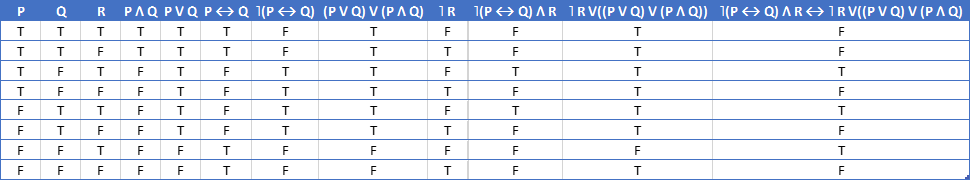
\includegraphics[width=.9\pagewidth]{p2-table}}

%	\newgeometry{top=.75in, bottom=.75in, left=.25in,right=.25in}
%	\newgeometry{top=.75in, bottom=.75in, left=1.25in,right=1.25in}

%	\lstinputlisting[firstline=4]{CMPSC360_Homework.cpp}

%\Tree
%	[.<root> [.<left> ][.<middle> ][.<right> ]]

%----------------------------------------------------------------------------------------
%	TITLE SECTION
%----------------------------------------------------------------------------------------

\newcommand{\horrule}[1]{\rule{\linewidth}{#1}} % Create horizontal rule command with 1 argument of height
% \title{Template: Homework 1}
\title{	
\normalfont \normalsize 
%\textsc{Rutgers University, Real Analysis I} \\ [25pt] % Your university, school and/or department name(s)
\horrule{0.5pt} \\[0.4cm] % Thin top horizontal rule
\huge STAT 463: Homework 2 \\ % The assignment title
\horrule{2pt} \\[0.5cm] % Thick bottom horizontal rule
}

\author{\textbf{\underline{Name:}}Kyle Salitrik | \textit{\textbf{\underline{ID\#:}} 997543474} | \textit{\textbf{\underline{PSU ID:}} kps168}} % Your name

\date{\normalsize\today} % Today's date or a custom date

\begin{document}

\maketitle % Print the title

%----------------------------------------------------------------------------------------
%	PROBLEM 1
%----------------------------------------------------------------------------------------
\newgeometry{top=.75in, bottom=.75in, left=1.25in,right=1.25in}
\section*{\variableheghtrulefill[.25ex]\quad Problem 1 \quad\variableheghtrulefill[.25ex]}

\subsection*{a)}
\makebox[\textwidth][c]{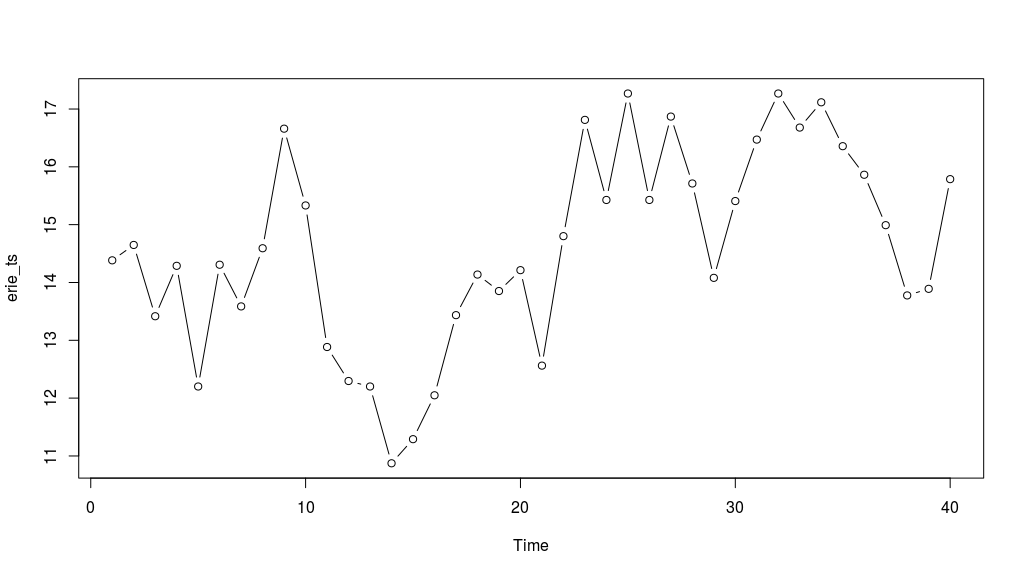
\includegraphics[width=\textwidth]{erie_timeseries.png}}

\subsection*{b)}
From the plot of the time series, point 14 could potentially be an outlier depending on who is looking at the data, but most likely is not. There is no seasonality to the data because it was collected yearly, however after year 20 the average does appear to increase. The variance is fairly constant from year 20 through 40.

\subsection*{c)}
\makebox[\textwidth][c]{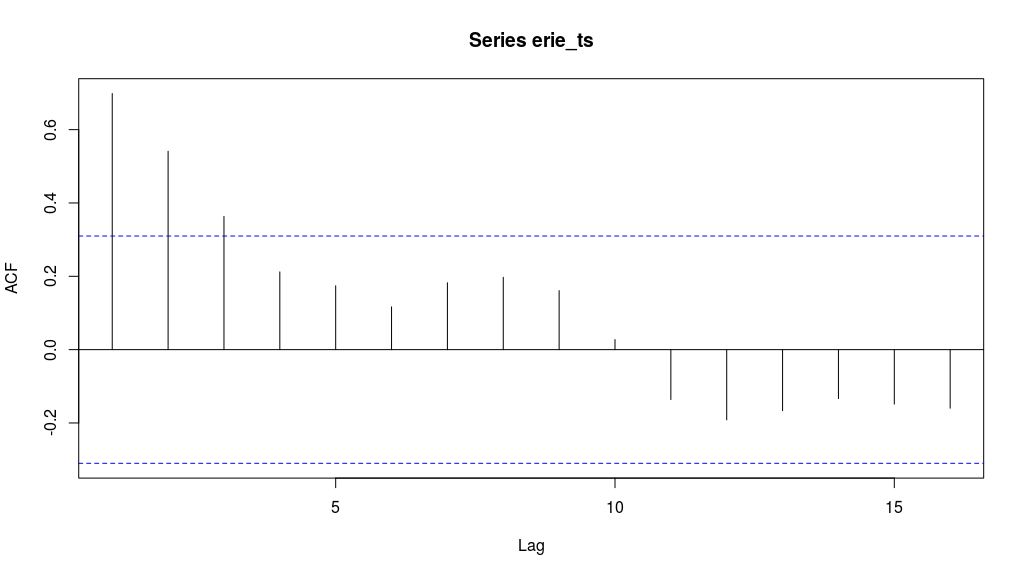
\includegraphics[width=\textwidth]{erie_acf.png}}

The first 5 or so values almost follow the theoretical curve. The table below summarizes the calculated and theoretical values, the absolute difference and the percentage difference from theoretical:

\begin{tabular}{| l | c | c | c | c | c | c | c |}
	\hline
	ACF Values & 0.698 & 0.541 & 0.363 & 0.212 & 0.174 & 0.117 & 0.182 \\ \hline
	Theoretical Values & 0.698 & 0.488 & 0.341 & 0.238 & 0.1662 & 0.1661 & 0.081 \\ \hline
	Absolute Difference & 0 & 0.053 & 0.022 & 0.026 & 0.008 & 0.001 & 0.101 \\ \hline
	Percentage Difference & 0\% & 9.829\% & 6.117\% & 12.220\% & 4.534\% & 0.634\% & 55.540\% \\ \hline
\end{tabular}

\subsection*{d)}
\lstinputlisting[language=]{listings/erie_lm_output.txt}
\begin{align*}
	\hat{y} &= 4.2878 + 0.7078x
\end{align*}

\subsection*{e)}	
The plot of residuals vs fitted values looks alright for a linear fitted model. The variance is mostly constant, there does not appear to be any trends in the data and the residuals themselves are fairly small ($\pm 2$) compared to the values of the water level (10.87 minimum, so less than a 20\% error at most for the residuals).

\makebox[\textwidth][c]{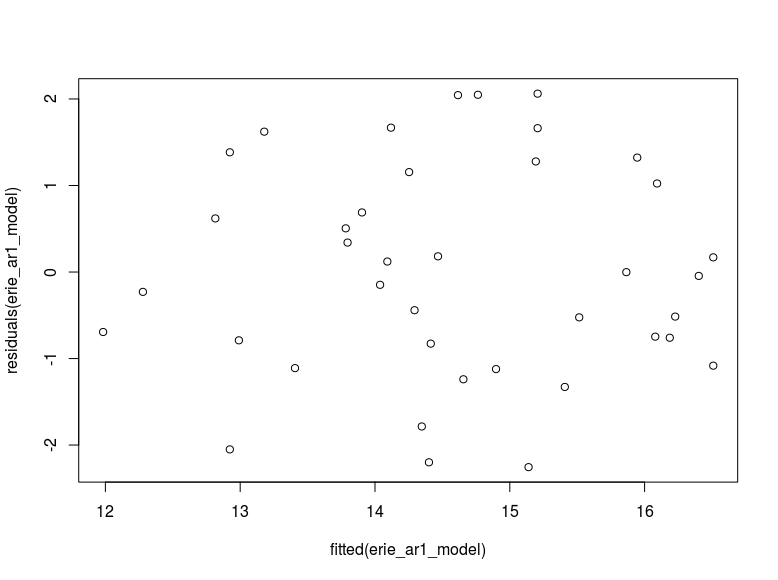
\includegraphics[width=.8\textwidth]{erie_res_vs_fit.png}}

\subsection*{f)}
From the plot of the residual ACF, because all of the residuals are within the confidence band, they appear to be affects of noise in the data.

\makebox[\textwidth][c]{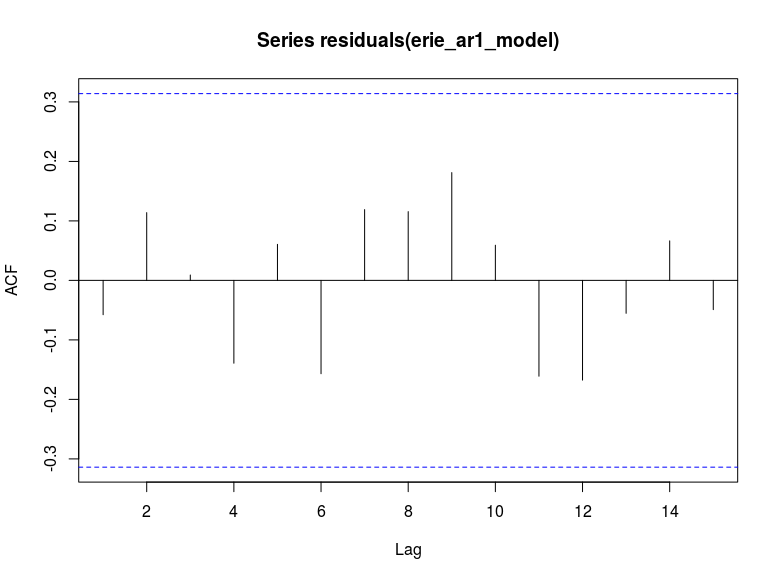
\includegraphics[width=.8\textwidth]{erie_residual_acf.png}}


\subsection*{g)}
$\hat{y}_{t=41} = 4.2878 + 0.7078*15.787 = 15.4618386$

%----------------------------------------------------------------------------------------
%	PROBLEM 2
%----------------------------------------------------------------------------------------

\section*{\variableheghtrulefill[.25ex]\quad Problem 2 \quad\variableheghtrulefill[.25ex]}
\subsection*{a)}
Based on the plot of the time series below, one piece of evidence that makes it safe to assume the series is not stationary is a non-constant mean.

\makebox[\textwidth][c]{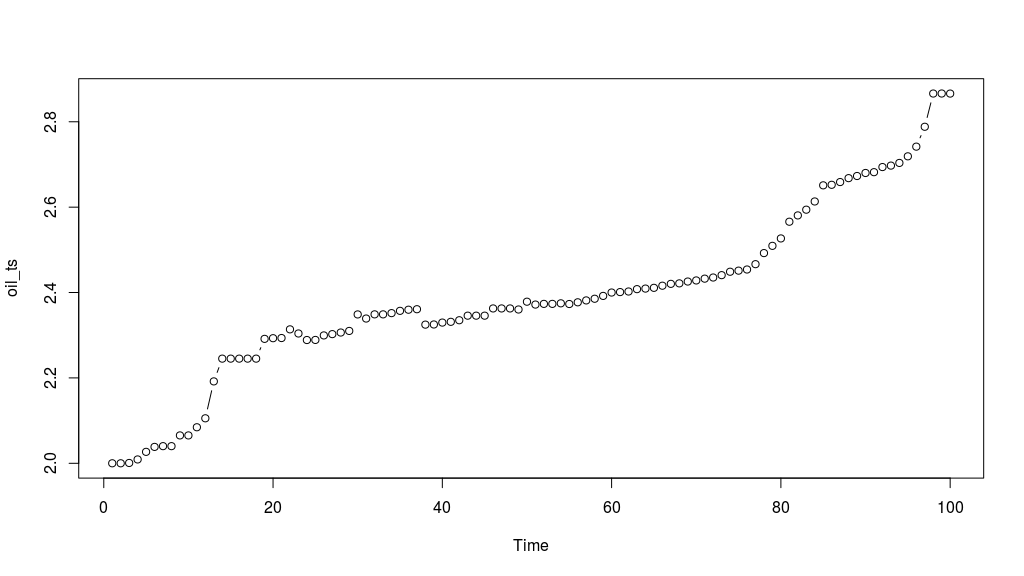
\includegraphics[width=\textwidth]{oil_timeseries.png}}


\subsection*{b)}
Observing the plot of the first differences of the data, with the exception of a few values that have a significantly large absolute value, the first difference is fairly constant at 0. The potential outliers referenced are at approximately points 13,14, 20, 30, 40, 97 and 98. However it is worth noting that the largest difference is 0.08 which is fairly close to 0.

\makebox[\textwidth][c]{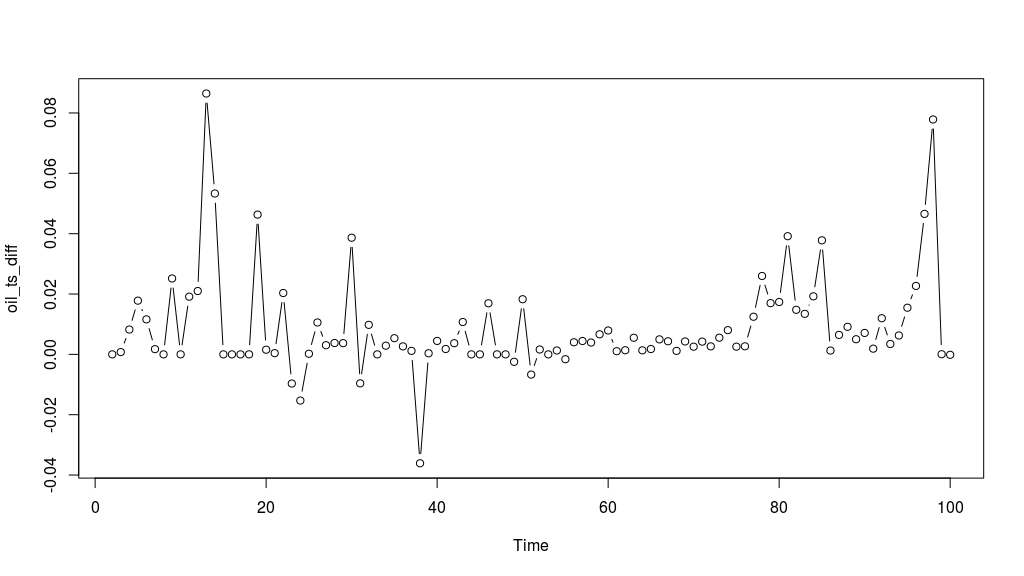
\includegraphics[width=\textwidth]{oil_first_diff.png}}

\subsection*{c)}
The R output is as follows:

\begin{tabular}{| c | c | c | c | c | c | c | c | c | c | c | c |}
	\hline
	1 & 2 & 3 & 4 & 5 & 6 & 7 & 8 & 9 & 10 & 11 & 12 \\ \hline
	0.317 & 0.082 & 0.061 & 0.059 & 0.028 & 0.080 & 0.059 & 0.027 & -0.007 & -0.048 & -0.042 & -0.080 \\ \hline
	13 & 14 & 15 & 16 & 17 & 18 & 19 &&&&&\\ \hline
	0.169 & 0.084 & 0.033 & 0.126 & 0.194 & 0.031 & -0.037 &&&&& \\ \hline
\end{tabular}

The plot below shows the ACF for the first differences. The plot doesn't appear to follow an AR(1) model because the drop off in magnitude seems too steep and the values are not constantly decreasing.

\makebox[\textwidth][c]{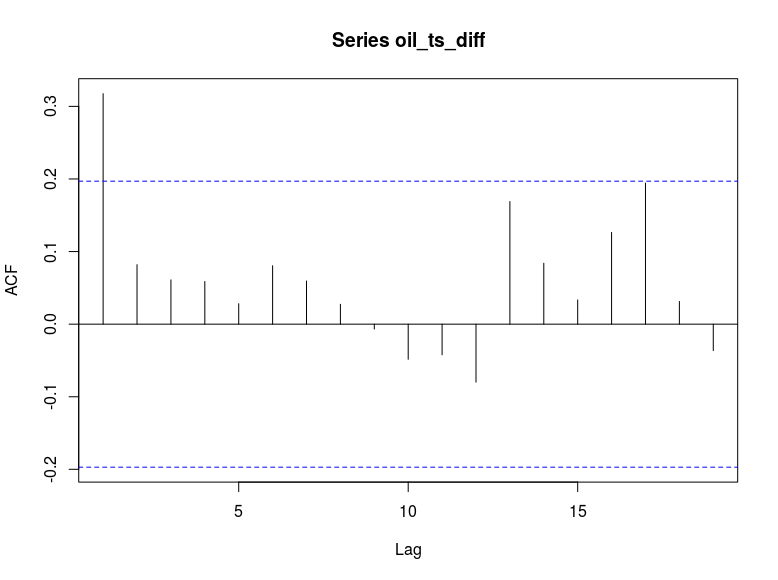
\includegraphics[width=\textwidth]{oil_diff_acf.png}}


\subsection*{d)}
The MA(1) model could potentially work because, as explained in class, the MA(1) model ACF plot should have a single spike in theory. However in practice the noisy data can cause small spikes further in the series. Because all of the values are within the confidence interval, they are considered to be close enough to 0 to be insignificant as true data and written off as noise.


%----------------------------------------------------------------------------------------
%	PROBLEM 3
%----------------------------------------------------------------------------------------

\section*{\variableheghtrulefill[.25ex]\quad Problem 3 \quad\variableheghtrulefill[.25ex]}

\subsection*{a)}

\makebox[\textwidth][c]{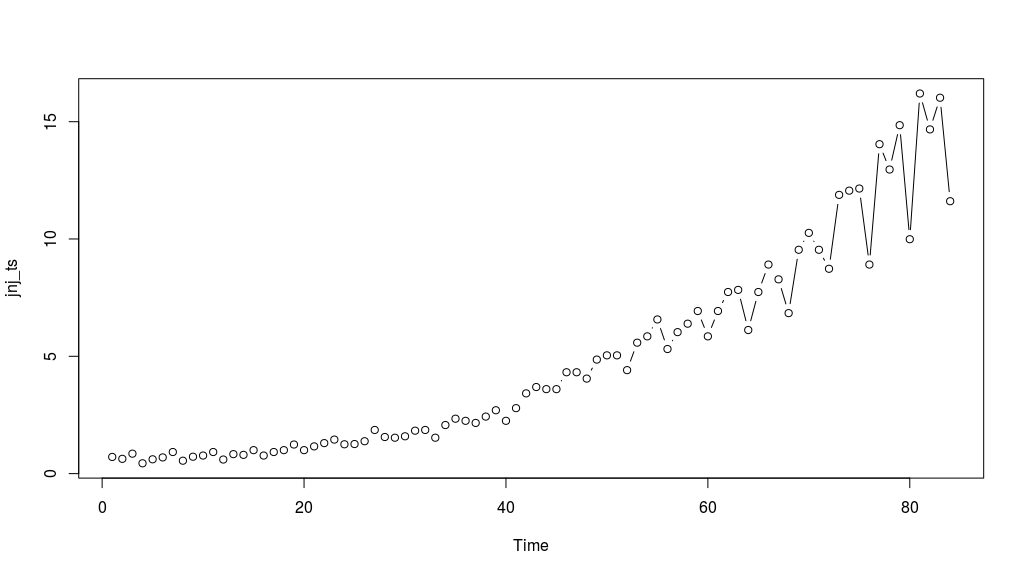
\includegraphics[width=\textwidth]{jnj_ts_plot.png}}


\subsection*{b)}
For the profit data, there appears to be a constant quadratic or exponential trend to the plot over time. Up until around t = 50, the variance is relatively constant, however it also begins to increase as time goes on.

\subsection*{c)}
Taking the logarithm of the profit values, the exponential trend is replaced with a linear one and the variance seems to be constant throughout the entire time period observed.

\makebox[\textwidth][c]{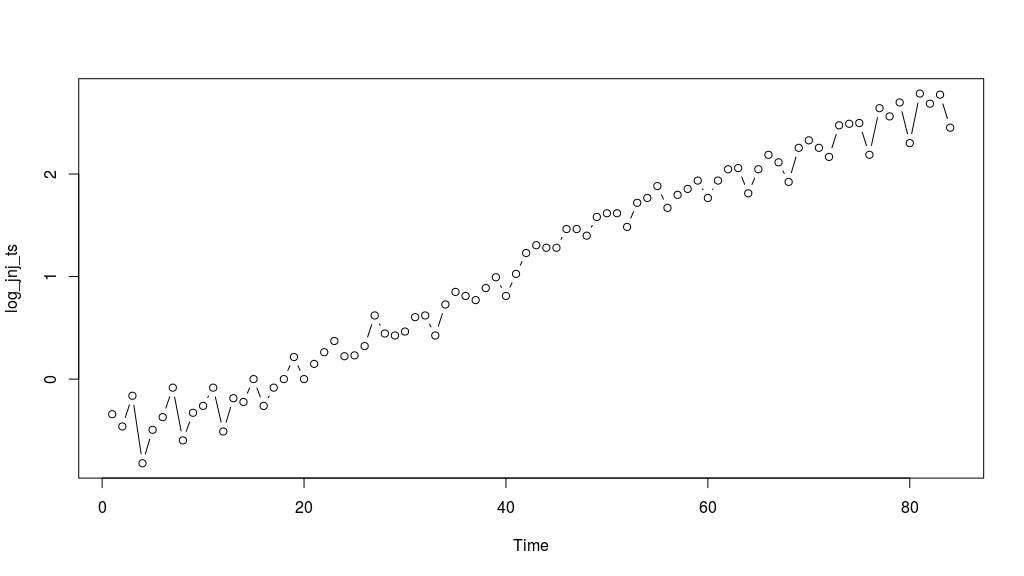
\includegraphics[width=\textwidth]{jnj_log_ts.png}}


\subsection*{d)}
If using a linear regression, the following model would most likely be a sufficient fit:
\begin{align*}
	log(\hat{y}) &= \beta_0 + \beta_1 * \text{profit}
\end{align*}


\end{document}